\chapter{Project tasks and resource allocation}

\begin{figure}
\centering
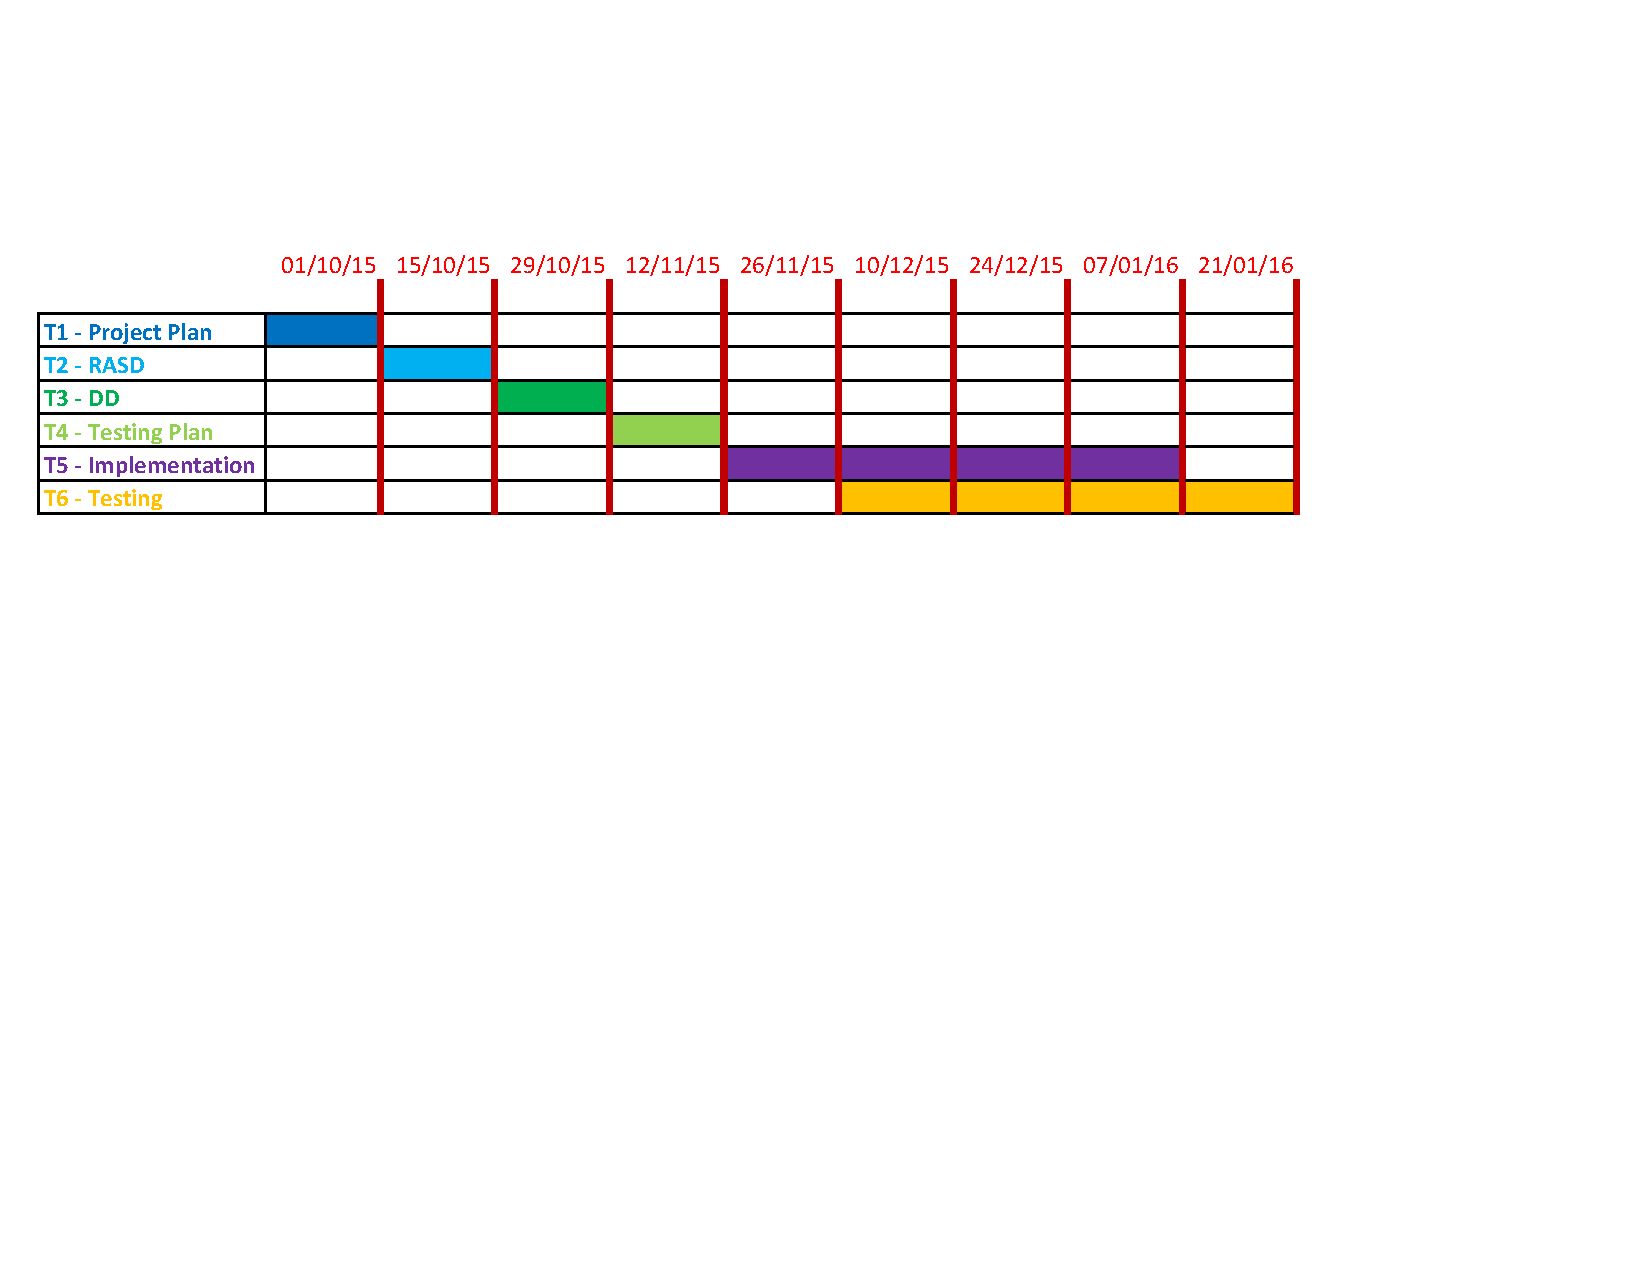
\includegraphics[width=\textwidth]{tex-images/TaskSchedule}
\caption{Task scheduling}
\end{figure}

\begin{figure}
\centering
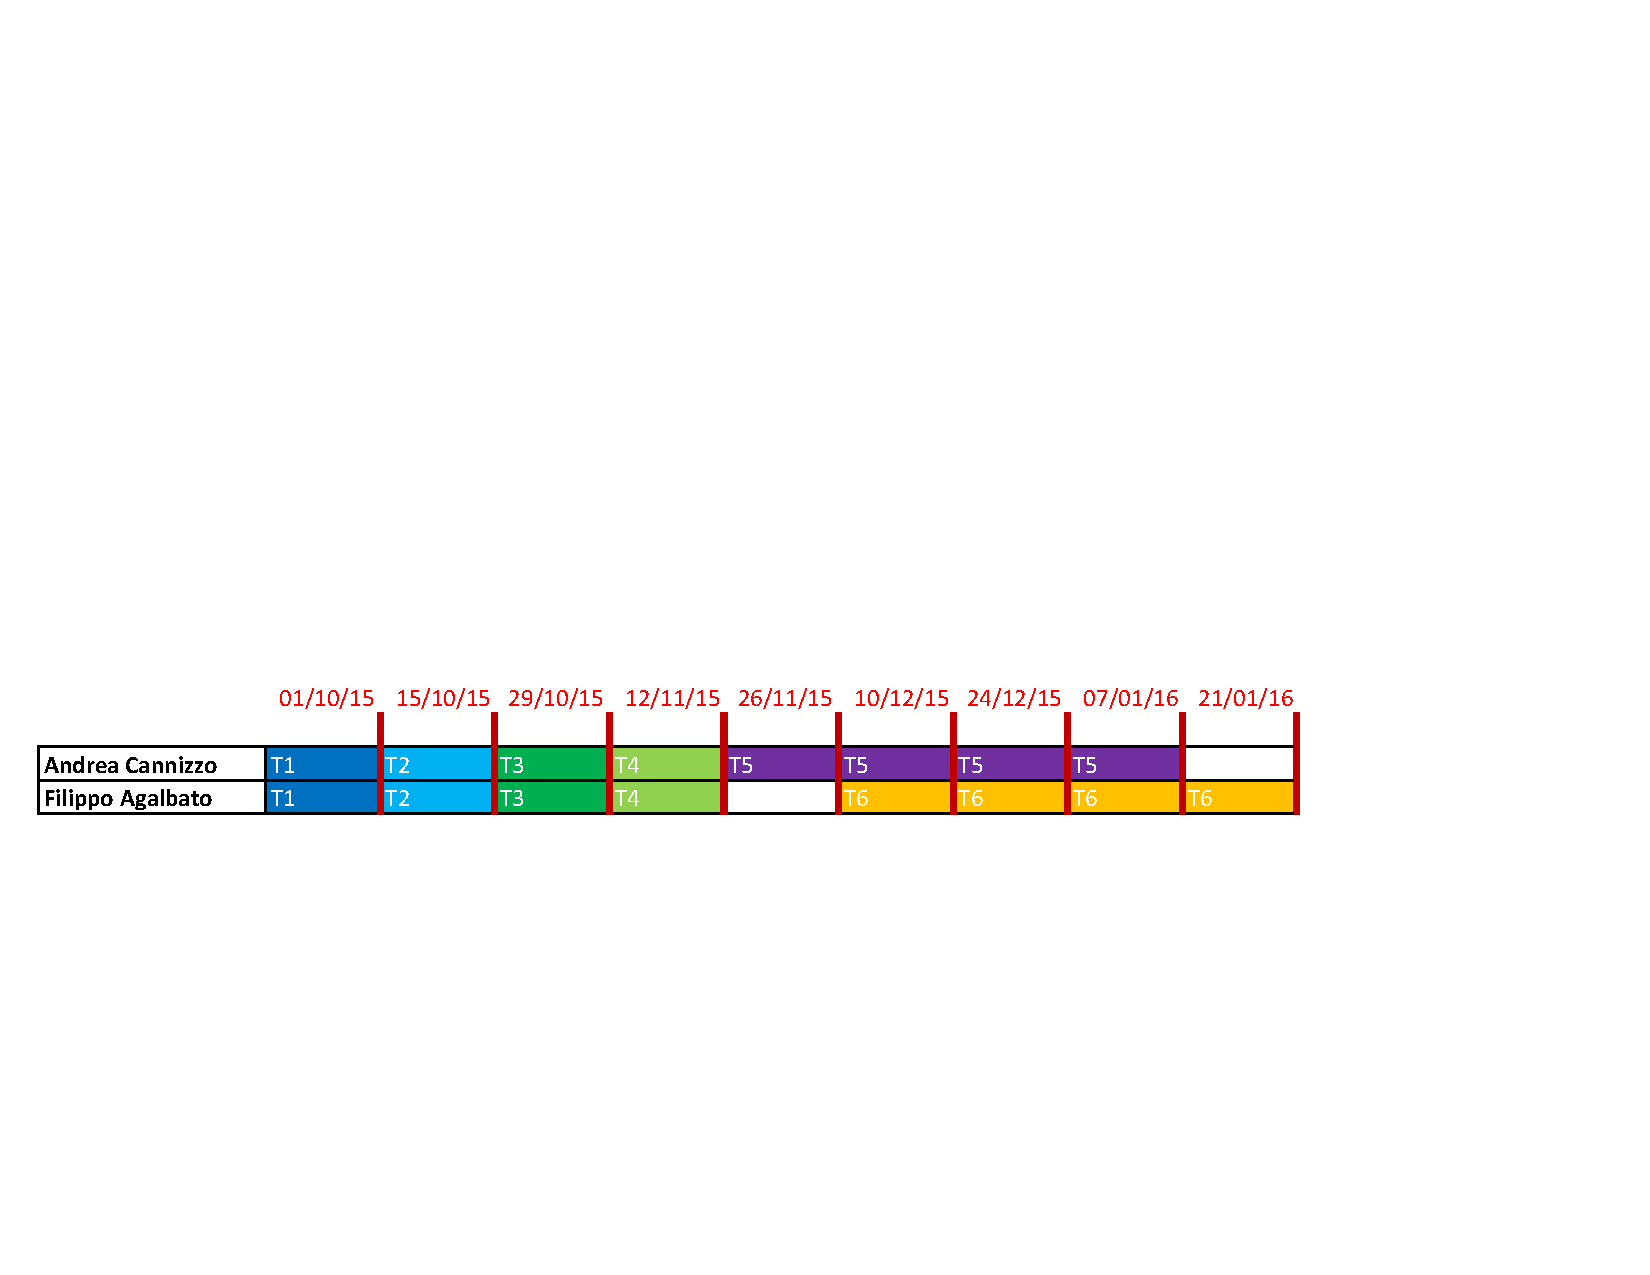
\includegraphics[width=\textwidth]{tex-images/ResourceAllocation}
\caption{Resource allocation}
\end{figure}

\section{Project Plan}
The elaboration of Project Plan document is the first step of Software Development.

\section{Requirement Analysis and Specification Document}
Elaboration of the Requirement Analysis and Specification Document. The goal of this document is to describe the system in terms of goals, requirements, assumptions and design, to define the different classes of users that will interact with it, and to analyse its most typical and most critical use cases. 
This document is targeted to the customer's project managers, to evaluate the project specification from a high-level point of view, and to the intended designers, developers, programmers, analysts and testers, to build the actual software and to maintain, integrate and expand it in the future. 

\section{Design Document}
Elaboration of Design Document. The goal of this document is to describe the system in term of architectural choices and design decisions, to provide an overview of the interactions between its components and the users, and to present samples of algorithmic pseudocode for the core systems. This document is targeted to the customer's project managers, to evaluate the project architecture from a high-level point of view, and to the intended designers, developers, programmers, analysts and testers, to build the actual software and to maintain, integrate and expand it in the future. 

\section{Testing Plan}
Elaboration of Testing Plan Document. The goal of this document is to describe the system's required integration testing framework and infrastructure that ought to prove its compliance with specifications, starting from these and proceeding up to the design phase of the different testing procedures. This document is targeted to the project testers, to correctly build their infrastructure so that the integration testing phase can proceed according to plan. 

\section{Implementation}
This task consists in writing source lines of code of the software using the chosen development language.

\section{Testing}
This task consists in testing the software following Testing Plan Document (Code Inspection, Unit Test, Integration Test, System Test, and so on).
